\documentclass[12pt,a4paper]{scrartcl} 
\usepackage[utf8]{inputenc}
\usepackage[english,russian]{babel}
\usepackage{indentfirst}
\usepackage{misccorr}
\usepackage{graphicx}
\usepackage{indentfirst}
\usepackage{amsmath}
\begin{document}
 \begin{titlepage}
  \begin{center}
   \large
   МИНИСТЕРСТВО НАУКИ И ВЫСШЕГО ОБРАЗОВАНИЯ РОССИЙСКОЙ ФЕДЕРАЦИИ
   
   Федеральное государственное бюджетное образовательное учреждение высшего образования
   
   \textbf{АДЫГЕЙСКИЙ ГОСУДАРСТВЕННЫЙ УНИВЕРСИТЕТ}
   \vspace{0.25cm}
   
   Инженерно-физический факультет
   
   Кафедра автоматизированных систем обработки информации и управления
   \vfill

   \vfill
   
   \textsc{Отчет по практике}\\[5mm]
   
   {\LARGE Программная реализация ранга матрицы. \textit{Вариант 6}}
   \bigskip
   
   1 курс, группа 1ИВТ1-2
  \end{center}
  \vfill
  
  \newlength{\ML}
  \settowidth{\ML}{«\underline{\hspace{0.7cm}}» \underline{\hspace{2cm}}}
  \hfill\begin{minipage}{0.5\textwidth}
   Выполнил:\\
   \underline{\hspace{\ML}} Н.\,С.~Сергеев\\
   «\underline{\hspace{0.7cm}}» \underline{\hspace{2cm}} 2023 г.
  \end{minipage}%
  \bigskip
  
  \hfill\begin{minipage}{0.5\textwidth}
   Руководитель:\\
   \underline{\hspace{\ML}} С.\,В.~Теплоухов\\
   «\underline{\hspace{0.7cm}}» \underline{\hspace{2cm}} 2023 г.
  \end{minipage}%
  \vfill
  
  \begin{center}
   Майкоп, 2023 г.
  \end{center}
 \end{titlepage}
 
% Содержание
\section{Введение}
\label{sec:intro}


\subsection{Формулировка цели}
Целью данной работы является написание программы для нахождение ранга матрицы.

\subsubsection{Теория}
Нахождение ранга матрицы способом элементарных преобразований
(методом Гаусса). Под элементарными преобразованиями матрицы понимаются
следующие операции:
    \begin{enumerate}
        \item умножение на число, отличное от нуля;
        \item прибавление к элементам какой-либо строки или какого-либо столбца;
        \item перемена местами двух строк или столбцов матрицы;
        \item удаление "нулевых" строк, то есть таких, все элементы которых равны нулю;
        \item удаление всех пропорциональных строк, кроме одной.
    \end{enumerate}
    \noindent 
Для любой матрицы A всегда можно прийти к такой матрице B,
вычисление ранга которой не представляет затруднений. Для этого следует
добиться, чтобы матрица B была трапециевидной. Тогда ранг полученной
матрицы будет равен числу строк в ней кроме строк, полностью состоящих из
нулей.

Ступенчатую матрицу называют трапециевидной или трапецеидальной,
если для ведущих элементов a1k1, a2k2, ..., arkr выполнены условия k1=1,
k2=2,..., kr=r, т.е. ведущими являются диагональные элементы. В общем виде
трапециевидную матрицу можно записать так:

\label{sec:picexample}
\begin{figure}[h]
 \centering
 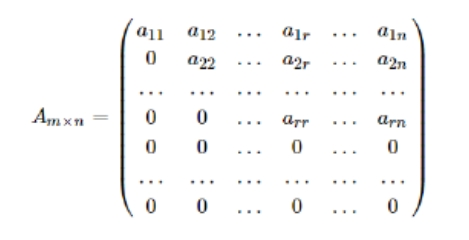
\includegraphics[width=0.5\textwidth]{theory.jpg}
    \caption{Трапециевидная матрица}\label{fig:par}

\end{figure}
\vfill
\newpage




\section{Ход работы}
\subsection{Код выполненной программы}
\begin{verbatim}

#include <iostream>
#include <vector>
#include <stdlib.h>
#include <Windows.h>
#include <cmath>
using namespace std;

int main()
{
	SetConsoleCP(1251);
	SetConsoleOutputCP(1251);
	int height, width, sum = 0, step = 0, sort1, sort2, rank; 
	int i, j, k, p, e;
	double tempmath, eps = 0.00001;
	cout << "Введите количество строк матрицы: ";
	cin >> height;
	cout << "Введите количество столбцов матрицы: ";
	cin >> width;
	if (height <= 0 || width <= 0)
	{
		cout << "Ошибка. Неверные параметры матрицы." << endl;
		return 0;
	}
	rank = height;
	vector <vector <double>> matrix;

	for (i = 0; i < height; i++)
	{
		vector <double> temp;
		for (j = 0; j < width; j++)
		{
			cout << "Введите элемент матрицы (" << i + 1 << ", " << j + 1 << "): ";
			cin >> e;
			temp.push_back(e);
		}
		matrix.push_back(temp);
	}
	cout << "\n";

    cout << "Заданная матрица: ";
	for (i = 0; i < height; i++)
	{
		for (j = 0; j < width; j++)
		{
			cout << matrix[i][j] << "\t";
		}
		cout << endl;
	}
	
	if (width > height - 1)
	{
		for (k = 0; k < height - 1; k++)
		{
			j = k;
			for (sort1 = k; sort1 < height; sort1++) {
				for (sort2 = k; sort2 < height - 1; sort2++) {
					if (abs(matrix[sort2][j]) < abs(matrix[sort2 + 1][j]))
					{
						for (j = 0; j < width; j++) swap(matrix[sort2][j], matrix[sort2 + 1][j]);
					}
					j = k;
				}
			}
			for (i = k + 1; i < height; i++)
			{
				j = k;
				tempmath = matrix[i][j] / matrix[i - 1 - step][j];
				if (matrix[i][j] == 0)
				{
					step++;
					continue;
				}
				else
				{
					for (j = k; j < width; j++)
					{
						matrix[i - step - 1][j] = matrix[i - step - 1][j] * tempmath;
						matrix[i][j] = matrix[i][j] - matrix[i - step - 1][j];
					}
					step++;
				}
			}
			step = 0;
			for (p = 0; p < width; p++)
				if (matrix[k + 1][p] == 0) sum++;
			if (sum == width)
			{
				for (p = 0; p < width; p++)
				{
					swap(matrix[height - 1][p], matrix[k + 1][p]);
				}
			}
			sum = 0;
		}
	}
	
	else
	{
		for (k = 0; k < width; k++)
		{
			j = k;
			for (sort1 = k; sort1 < height; sort1++) {
				for (sort2 = k; sort2 < height - 1; sort2++) {
					if (matrix[sort2][j] < matrix[sort2 + 1][j])
					{
						for (j = 0; j < width; j++) swap(matrix[sort2][j], matrix[sort2 + 1][j]);
					}
					j = k;
				}
			}
			for (i = k + 1; i < height; i++)
			{
				j = k;
				tempmath = matrix[i][j] / matrix[i - 1 - step][j];
				if (matrix[i][j] == 0)
				{
					step++;
					continue;
				}
				else
				{
					for (j = k; j < width; j++)
					{
						matrix[i - step - 1][j] = matrix[i - step - 1][j] * tempmath;
						matrix[i][j] = matrix[i][j] - matrix[i - step - 1][j];
					}
					step++;
				}
			}
			step = 0;
			for (p = 0; p < width; p++)
				if (matrix[k + 1][p] == 0) sum++;
			if (sum == width)
			{
				for (p = 0; p < width; p++)
				{
					swap(matrix[height - 1][p], matrix[k + 1][p]);
				}
			}
			sum = 0;
		}
	}
	for (i = 0; i < height; i++)
	{
		for (j = 0; j < width; j++)
		{
			if (abs(matrix[i][j]) < eps) matrix[i][j] = 0;
		}
	}
	cout << "\nПриведенная матрица:" << endl;
 
	for (i = 0; i < height; i++)
	{
		for (j = 0; j < width; j++)
		{
			cout << matrix[i][j] << "\t";
		}
		cout << endl;
	}
 
	for (i = 0; i < height; i++)
	{
		for (j = 0; j < width; j++)
		{
			if (matrix[i][j] == 0) sum++;
		}
		if (sum == width) rank--;
		sum = 0;
	}

	cout << "\nРанг матрицы: " << rank;

	return 0;
}	

\end{verbatim}

\begin{figure}[h]
 \centering
 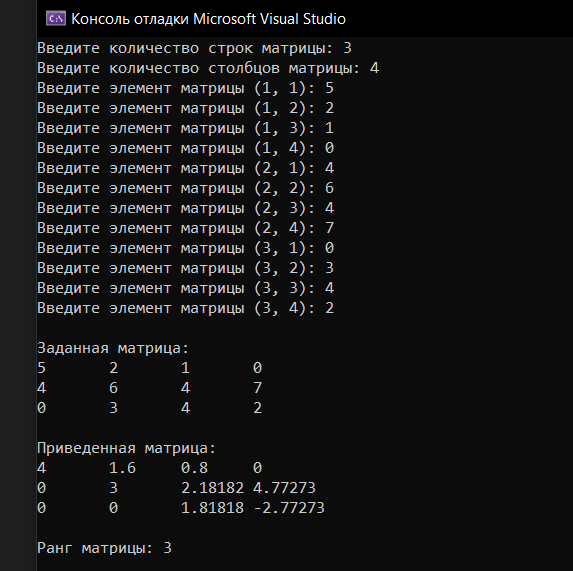
\includegraphics[width=0.8\textwidth]{result.png}
 \caption{Результат работы}\label{fig:par}
\end{figure}

\end{document}